\mychapter{Resultados}{chp:resultados}
\lhead{RESULTADOS}


\begin{center}
	\fbox{
	\colorbox[RGB]{227, 227, 227}{
	\parbox[t]{.8\linewidth}
		{Neste capítulo tratamos os resultados esperados com a realização do trabalho enquanto que no próximo faremos a conclusão alcançada com o mesmo.}} }
\end{center}

Para cada gerador considerado, cada tamanho de palavra e cada \textit{lag} coletamos \num{52429} sequências disjuntas.
Cada sequência passou pelo processo de simbolização, e foi calculado o histograma dos símbolos.
Foram então calculados os valores de Entropia e de Complexidade de cada histograma, bem como a distância euclidiana desses valores ao ponto de referência $(1,0)$.

Acompanhando a análise realizada por \citet{NewPermutationEntropy}, calculamos os valores máximo e mínimo, bem como os quantis de ordem $1/1000$, $1/100$, $5/100$ e $10/100$ (arredondadas) das distâncias.

\section{Análise das sequências quânticas}

A figura~\ref{Fig:ScatterAllQuantic} mostra os planos Entropia-Complexidade com as respectivas curvas de complexidade mínima e máxima para cada par $D\in\{3,4,5,6\}$ (colunas) e $\tau\in\{1,10,30,50\}$ (linhas), com os \num{52429} pontos observados.
Os pontos foram desenhados com \SI{1}{\percent} de transparência, para evidenciar as regiões mais e menos densas.

\begin{figure}[hbt]
\centering
\includegraphics[width=\linewidth]{../Plots/ScatterAllQuantic}
\caption{Diagramas de dispersão das sequências quânticas para $D\in\{3,4,5,6\}$ (colunas) e $\tau\in\{1,10,30,50\}$ (linhas), com curvas de complexidade mínima e máxima no plano Entropia-Complexidade.}\label{Fig:ScatterAllQuantic}
\end{figure}

Antes de analisar os diagramas de dispersão, analisaremos a distribuição empírica das distâncias ao ponto de referência.

\begin{figure}[hbt]
\centering
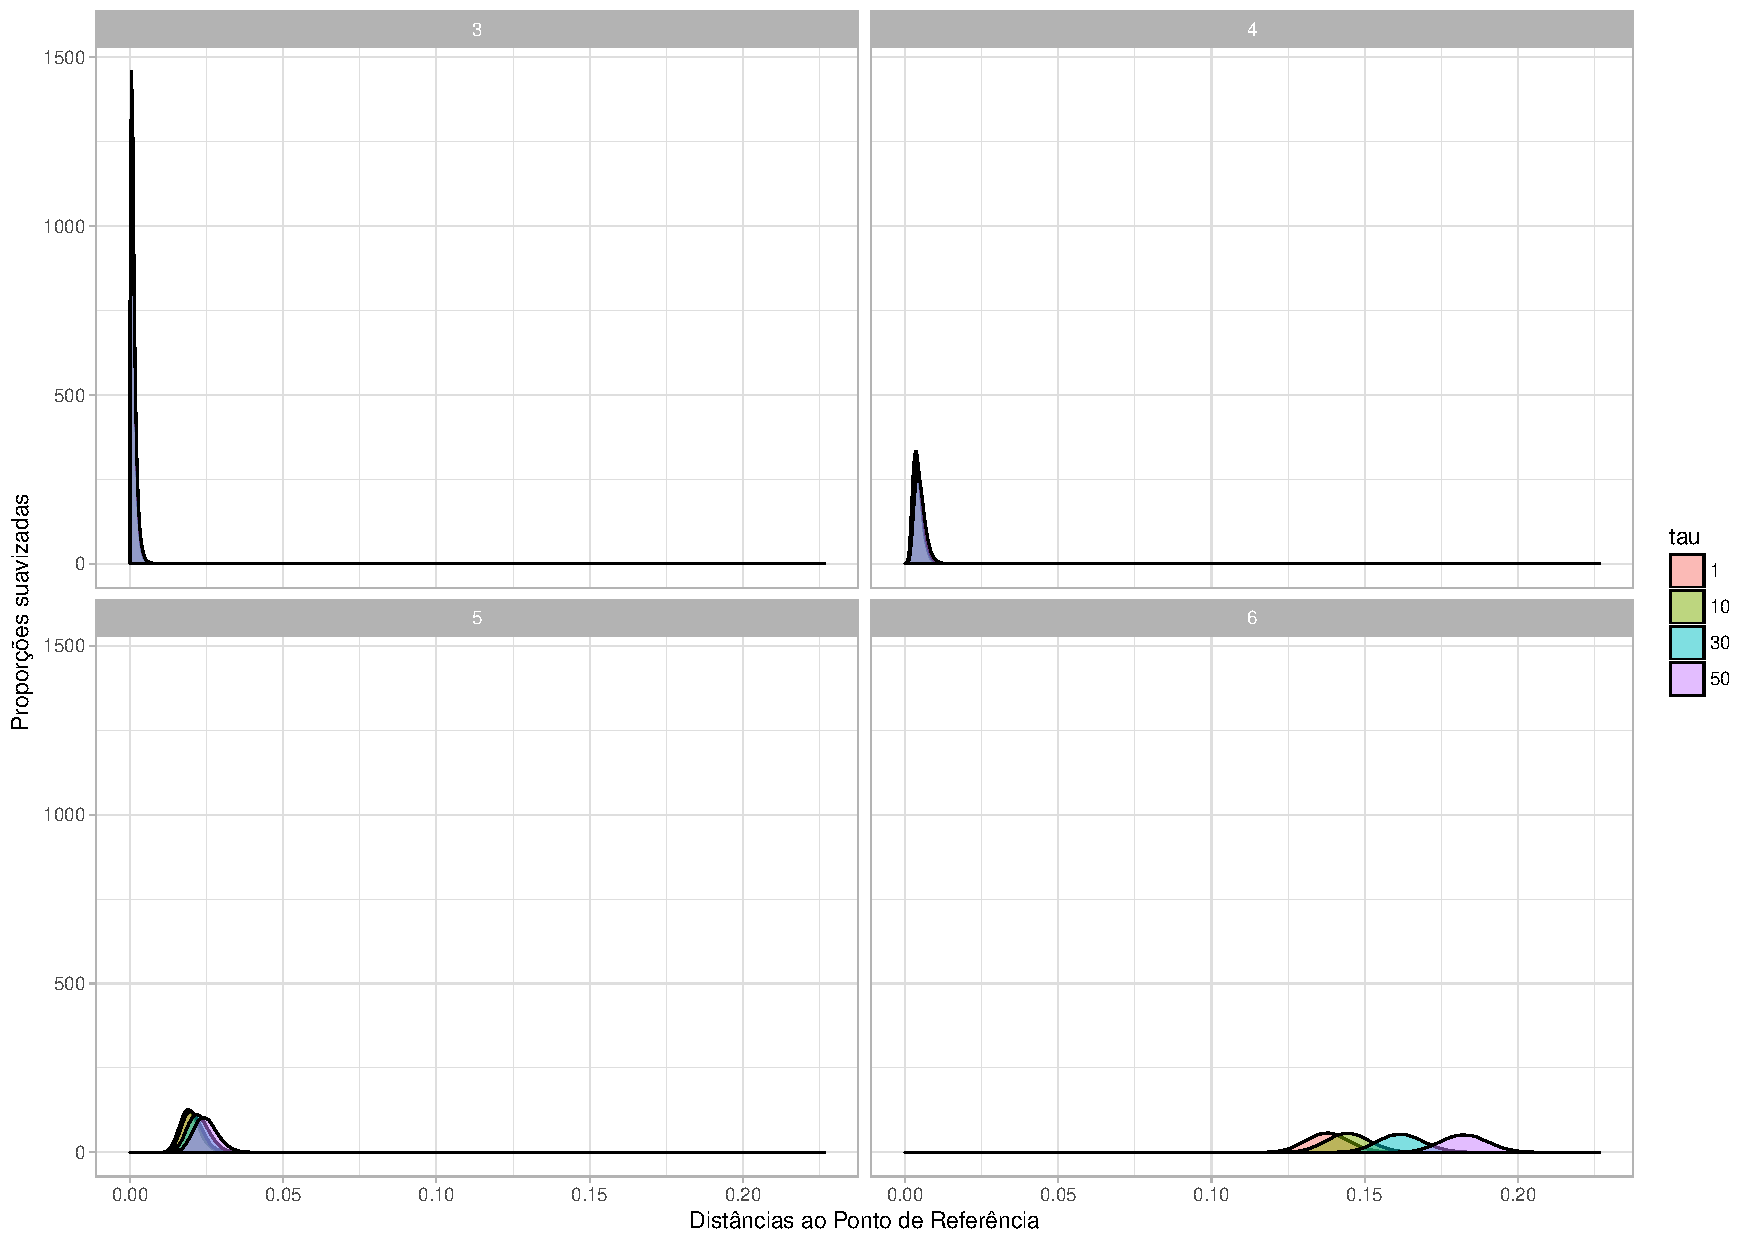
\includegraphics[width=\linewidth]{../Plots/HistoDistanciasQuantTodas}
\caption{Histogramas suavizados das distâncias euclidianas dos padrões ao ponto de referência, para $D\in\{3,4,5,6\}$ (colunas) e $\tau\in\{1,10,30,50\}$ (linhas).}\label{Fig:HistoDistanciasQuantTodas}
\end{figure}

A figura~\ref{Fig:HistoDistanciasQuantTodas} sugere que o comportamento das distâncias euclidianas ao ponto de referência muda conforme o tamanho do padrão $D$ varia.
Além disso, também são perceptíveis mudanças de comportamento em funçao do \textit{lag} $\tau$ quando $D=5,6$.

No que segue analisaremos o comportamento dessas distâncias em detalhes.


\begin{figure}
\centering
\subfigure[Escala linear\label{Fig:ScatterQuantD3tau1}]{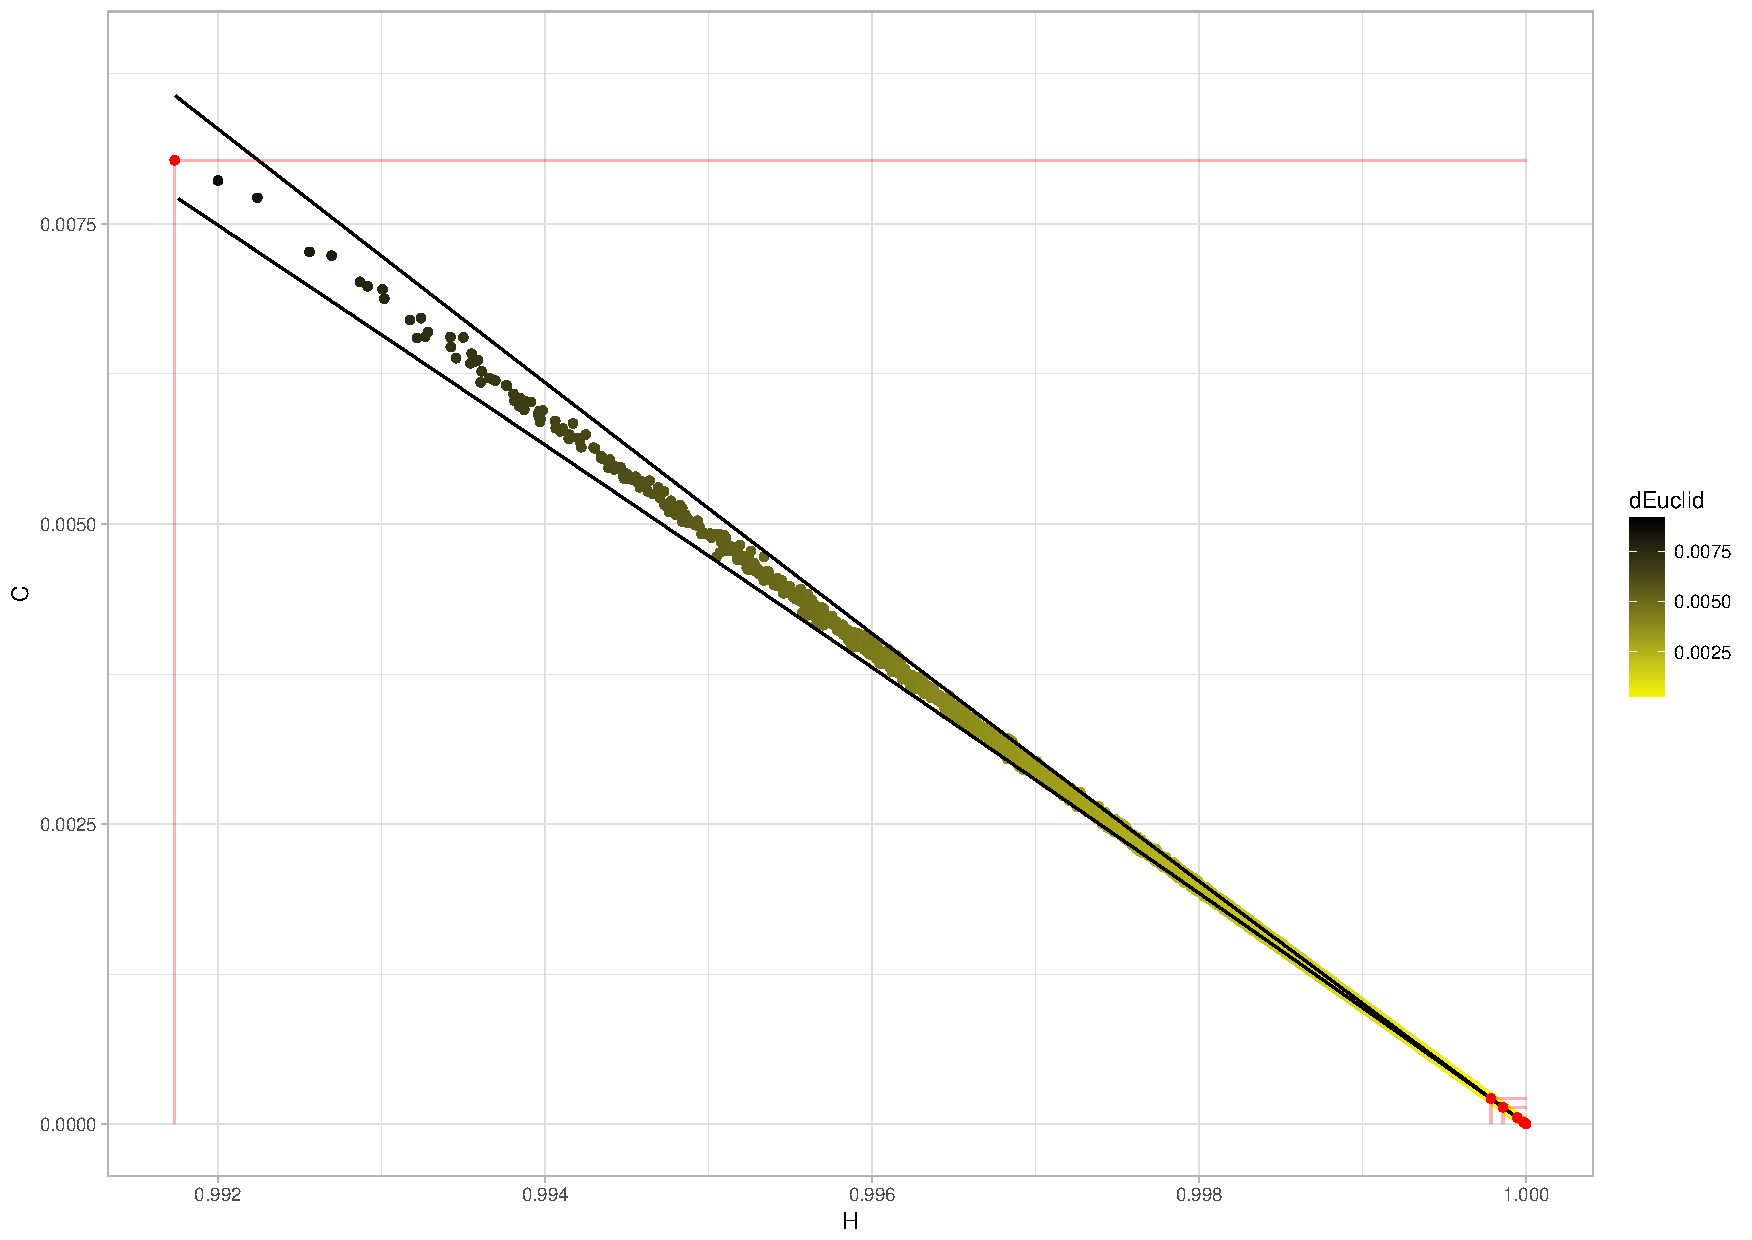
\includegraphics[width=.48\linewidth]{../Plots/ScatterQuantD3tau1}}
\subfigure[Escala logarítmica\label{Fig:ScatterQuantD3tau1log}]{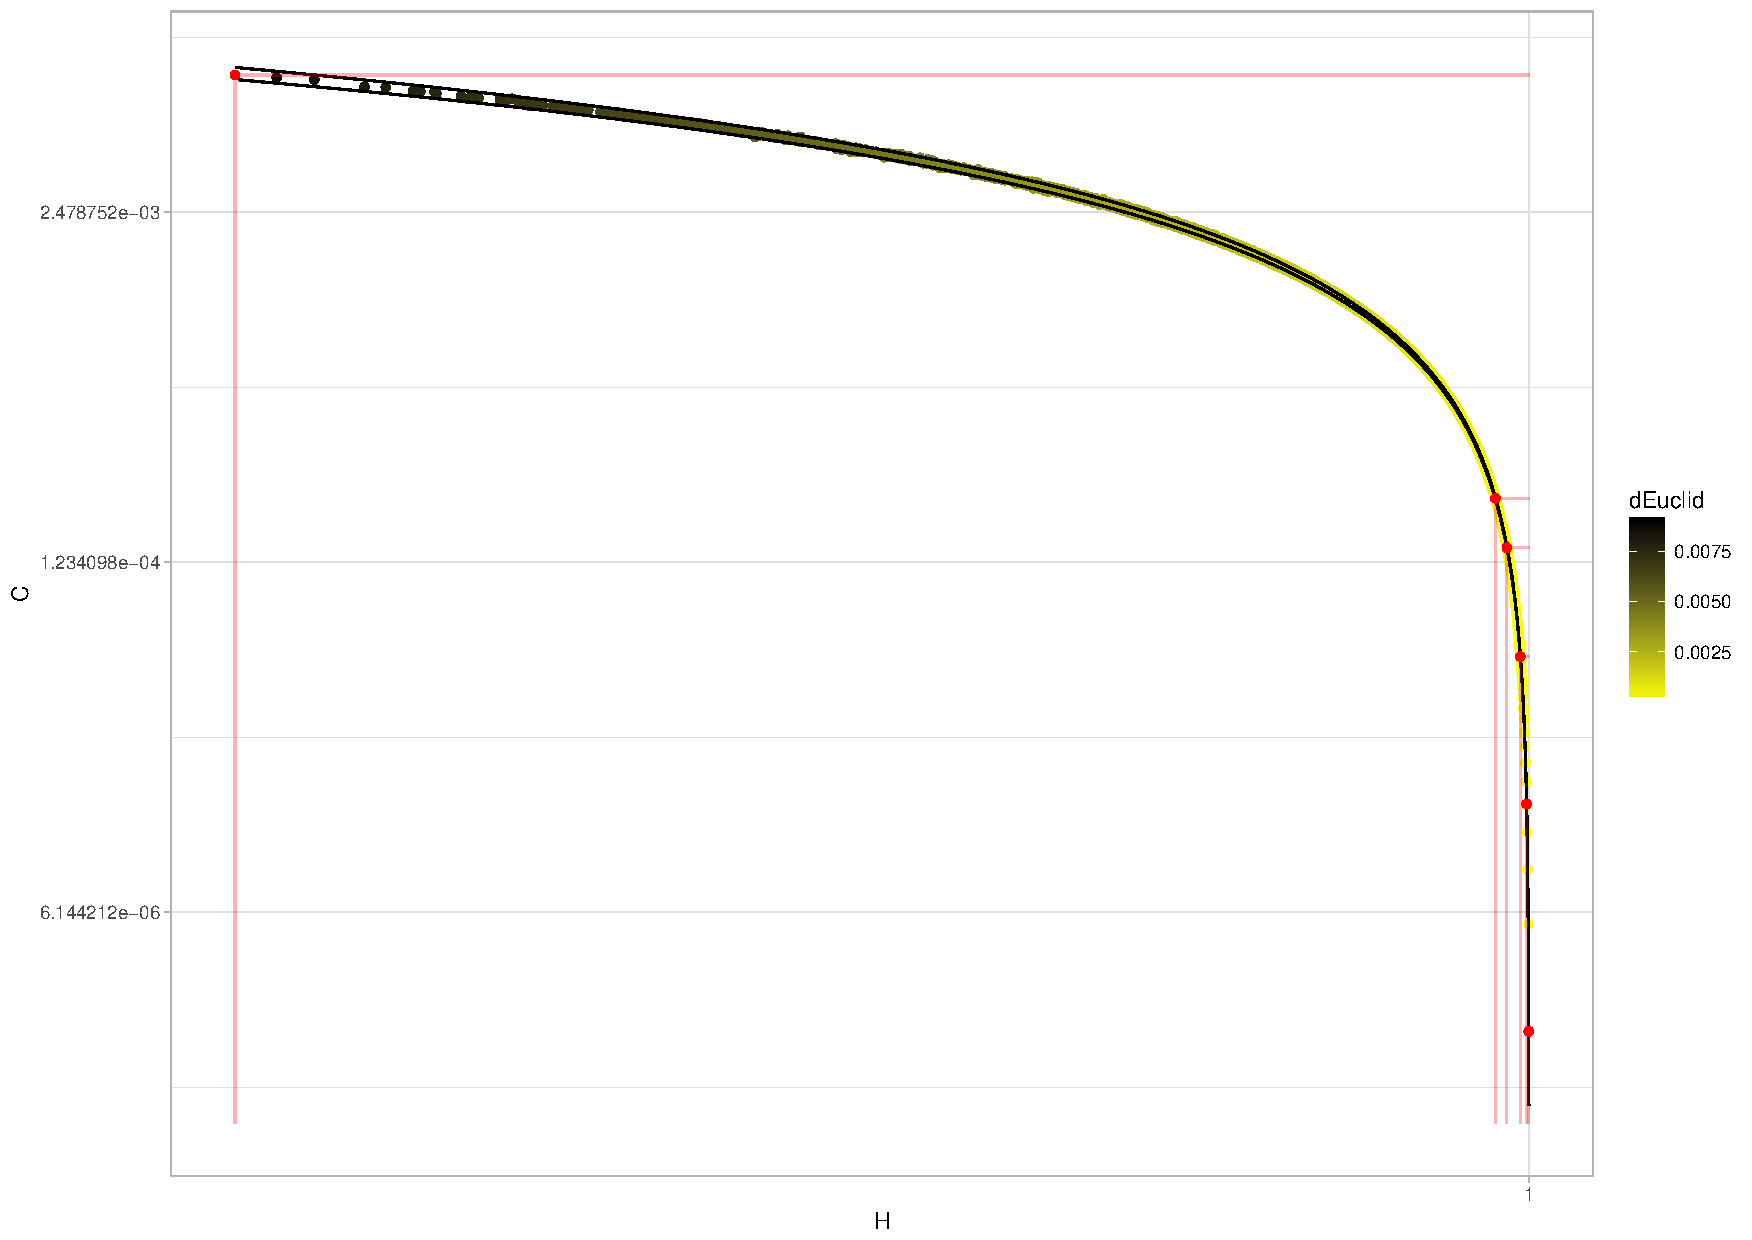
\includegraphics[width=.48\linewidth]{../Plots/ScatterQuantD3tau1log}}
\caption{Diagramas de dispersão das sequências quânticas para o caso $D=3$ e $\tau=1$.}\label{Fig:QuantD3tau1}
\end{figure}

\begin{figure}
\centering
\subfigure[Escala linear\label{Fig:ScatterQuantD3tau10}]{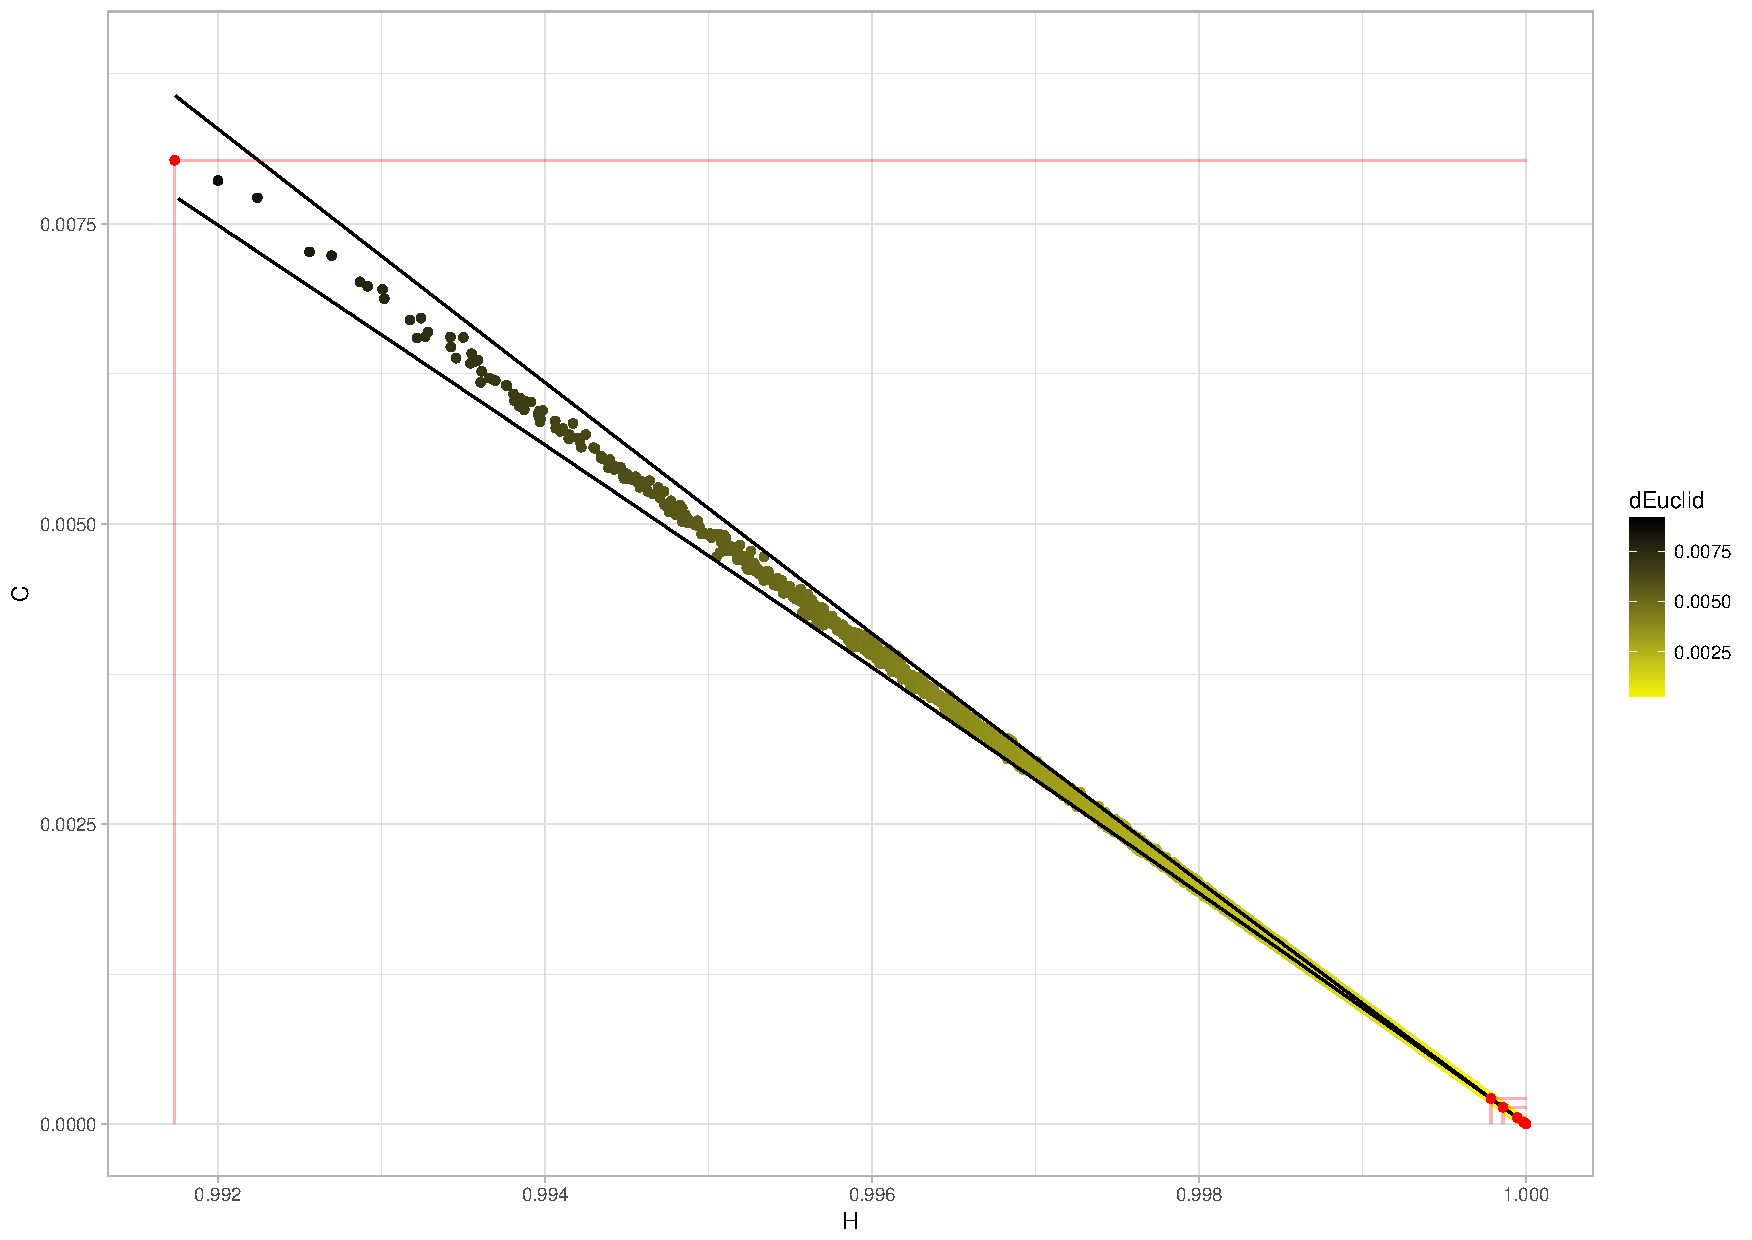
\includegraphics[width=.48\linewidth]{../Plots/ScatterQuantD3tau1}}
\subfigure[Escala logarítmica\label{Fig:ScatterQuantD3tau10log}]{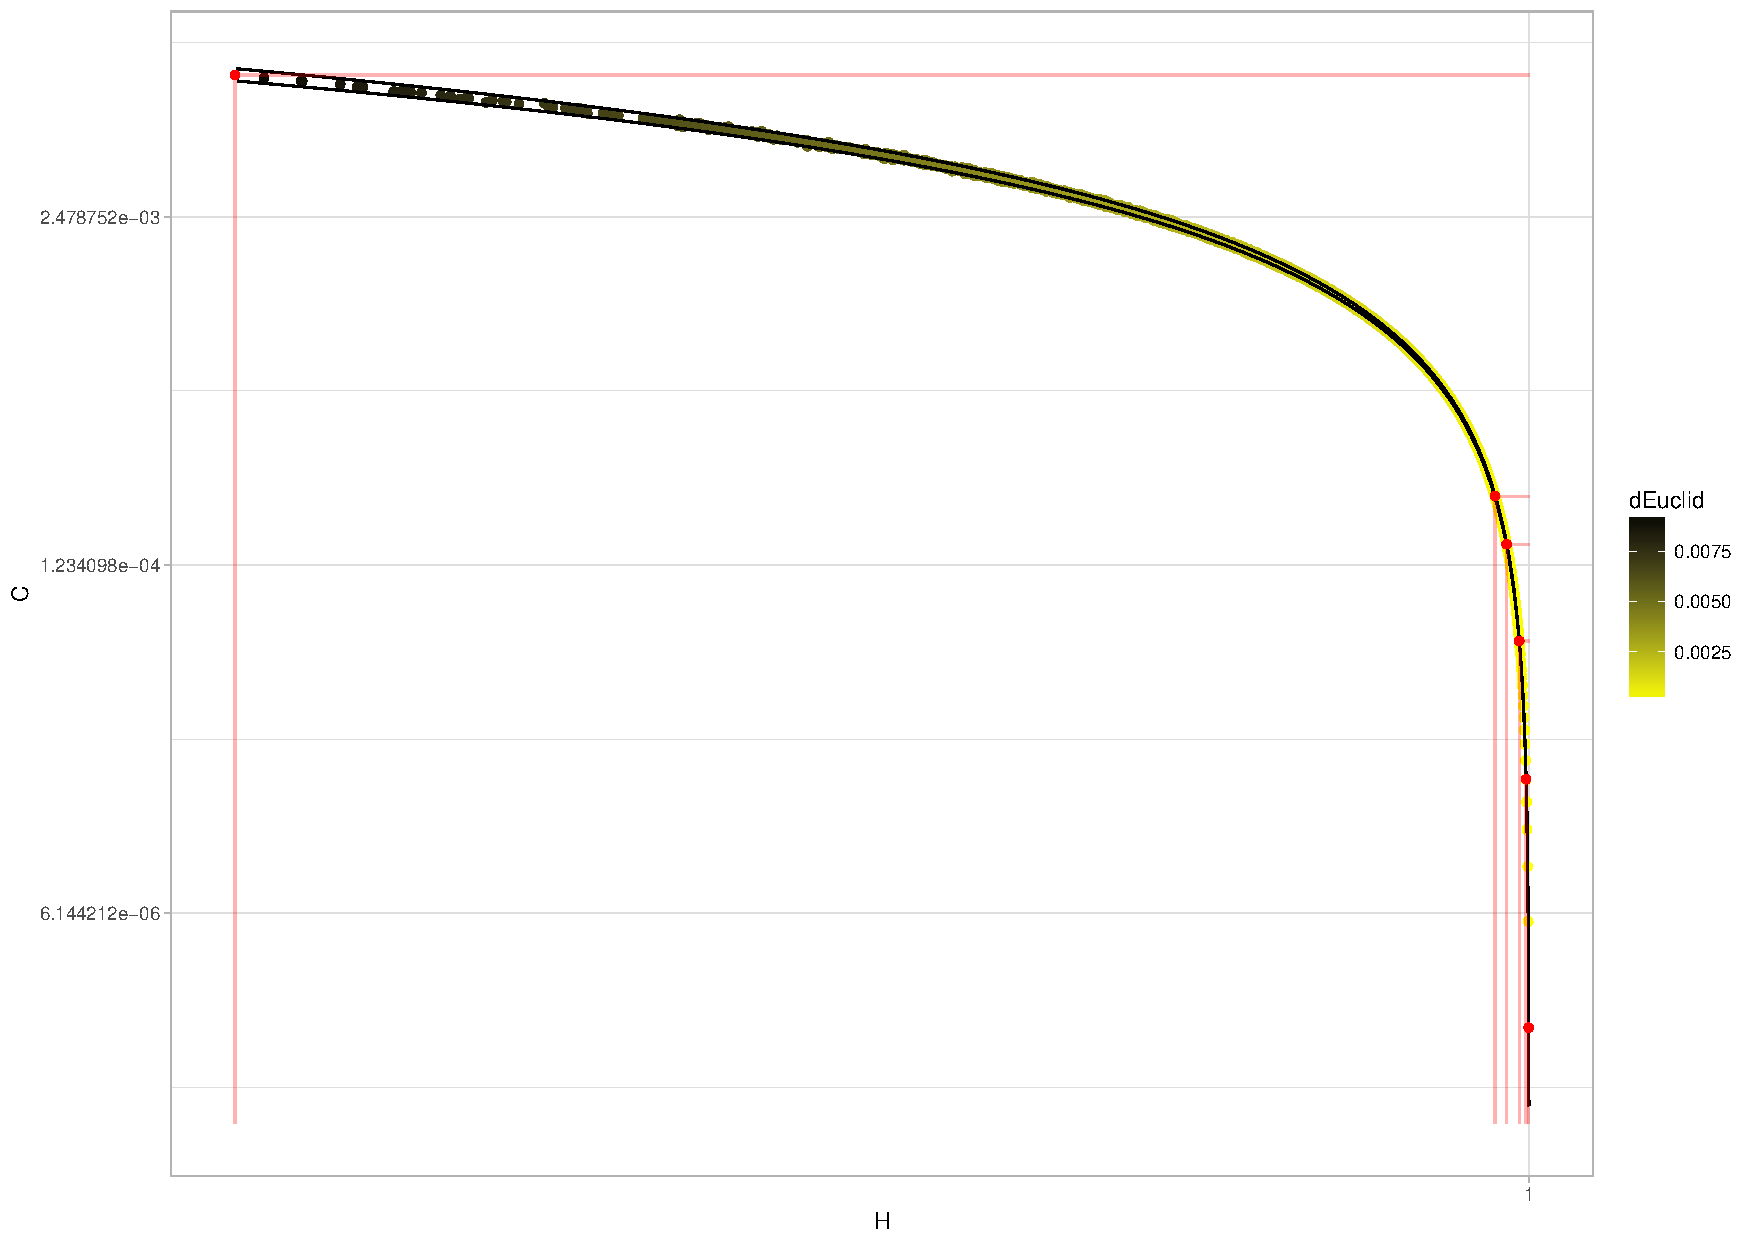
\includegraphics[width=.48\linewidth]{../Plots/ScatterQuantD3tau10log}}
\caption{Diagramas de dispersão das sequências quânticas para o caso $D=3$ e $\tau=10$.}\label{Fig:QuantD3tau10}
\end{figure}


Constatamos notáveis diferenças na distribuição espacial dos pontos segundo o tamanho da palavra $D$, fato que motiva a análise detalhada de cada situação.

\section{Análise das sequências de rádio}

\section{Análise das sequências Mersenne-Twister}




